\documentclass{article}
\usepackage[utf8x]{inputenc}
\usepackage{ucs}
\usepackage{amsmath} 
\usepackage{amsfonts}
\usepackage{upgreek}
\usepackage[english,russian]{babel}
\usepackage{graphicx}
\usepackage{float}
\usepackage{textcomp}
\usepackage{hyperref}
\usepackage{geometry}
  \geometry{left=2cm}
  \geometry{right=1.5cm}
  \geometry{top=1cm}
  \geometry{bottom=2cm}
\usepackage{tikz}
\usepackage{ccaption}
\usepackage{multicol}

\usepackage{listings}
%\setlength{\columnsep}{1.5cm}
%\setlength{\columnseprule}{0.2pt}


\begin{document}
\pagenumbering{gobble}

\lstset{
  language=C++,                % choose the language of the code
  basicstyle=\linespread{1.1}\ttfamily,
  columns=fixed,
  fontadjust=true,
  basewidth=0.5em,
  keywordstyle=\color{blue}\bfseries,
  commentstyle=\color{gray},
  stringstyle=\ttfamily\color{orange!50!black},
  showstringspaces=false,
  %numbers=false,                   % where to put the line-numbers
  numbersep=5pt,
  numberstyle=\tiny\color{black},
  numberfirstline=true,
  stepnumber=1,                   % the step between two line-numbers.        
  numbersep=10pt,                  % how far the line-numbers are from the code
  backgroundcolor=\color{white},  % choose the background color. You must add \usepackage{color}
  showstringspaces=false,         % underline spaces within strings
  captionpos=b,                   % sets the caption-position to bottom
  breaklines=true,                % sets automatic line breaking
  breakatwhitespace=true,         % sets if automatic breaks should only happen at whitespace
  xleftmargin=.2in,
  extendedchars=\true,
  keepspaces = true,
}
\lstset{literate=%
   *{0}{{{\color{red!20!violet}0}}}1
    {1}{{{\color{red!20!violet}1}}}1
    {2}{{{\color{red!20!violet}2}}}1
    {3}{{{\color{red!20!violet}3}}}1
    {4}{{{\color{red!20!violet}4}}}1
    {5}{{{\color{red!20!violet}5}}}1
    {6}{{{\color{red!20!violet}6}}}1
    {7}{{{\color{red!20!violet}7}}}1
    {8}{{{\color{red!20!violet}8}}}1
    {9}{{{\color{red!20!violet}9}}}1
}


\title{Семинар \#2: Библиотека SFML. Событийно-ориентированное программирование. Классные задачи.\vspace{-5ex}}\date{}\maketitle
\begin{itemize}
\item \textbf{Фигуры}: В SFML есть несколько классов для работы с простыми фигурами: \texttt{sf::CircleShape} (круг или элипс), \texttt{sf::RectangleShape} (прямоугольник), \texttt{sf::ConvexShape}(фигура сложной формы, задаваемая точками). У этих классов есть общие методы:
\begin{itemize}
\item \texttt{setOrigin} - установить центр фигуры (по умолчанию -- верхний левый угол)
\item \texttt{setPosition}, \texttt{getPosition} - задать и получить координаты центра
\item \texttt{move} - принимает 2D вектор и передвигает фигуру на этот вектор
\item \texttt{setRotation}, \texttt{getRotation} - задать и получить угол вращения
\item \texttt{rotate} - принимает вещественное число и вращает фигуру на этот угол (в градусах)
\item \texttt{setScale}, \texttt{getScale} - задать и получить величину масштабирования (2D вектор)
\item \texttt{scale} - принимает  2D вектор и растягивает или сжимает фигуру по x и по y соответственно
\item \texttt{setFillColor}, \texttt{getFillColor} -- устанавливает цвет
\end{itemize}
В папке \texttt{0shapes} приведён пример программы, которая рисует несколько фигур. Используйте методы выше и сделайте так, чтобы круг двигался по прямой, прямоугольник вращался, а фигура сложной формы сжималась по y и растягивалась по x. Подберите скорости этих операций, чтобы они были не слишком быстрыми.

\item \textbf{Anti-Aliasing}:
\begin{multicols}{2}
\begin{center}
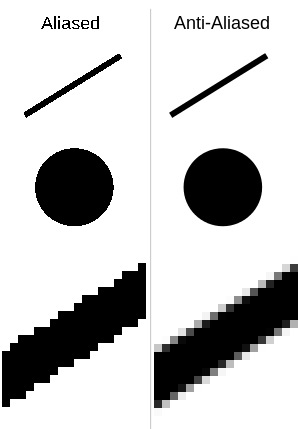
\includegraphics[scale=0.5]{../images/anti-aliasing.png}
\end{center}
Вы могли заметить, что фигуры выглядят не очень красиво - имеют зазубрены. Это связано с тем, что рисования происходит на прямоугольной сетке пикселей и при проведении линий под углом образуются ступеньки. Для борьбы с этим эффектом был придуман специальный метод сглаживания, который называется антиалиасинг. Он уже автоматически реализован во всех библиотеках компьютерной графики. Чтобы установить его в SFML, нужно прописать опцию:
\begin{lstlisting}
sf::ContextSettings settings;
settings.antialiasingLevel = 8;
\end{lstlisting}
И передать \texttt{settings} на вход для конструктора \texttt{RenderWindow}.
\end{multicols}
Протестируйте программу с разными уровнями антиалиасинга.

\item \textbf{Кадры в секунду:} Сейчас основной цикл программы работает без перерывов и, так как наша программа очень проста, то количество кадров в секунды(fps) может достигать огромных значений - больше 1000 fps. Мониторы не обновляют экран с такой скоростью и человеческий глаз тоже не способен воспринять такую частоту кадров. Поэтому не имеет смысла задавать fps очень высоким. Ограничьте число кадров в секунду 60-ю с помощью метода \texttt{setFramerateLimit} класса \texttt{RenderWindow}.

\item \textbf{KeyPressed:} В папке \texttt{1key\_events} лежит пример программы, которая обрабатывает нажатия клавиш. Измените программу так, чтобы при нажатии на клавишу Enter кружок менял цвет на случайный.

\item \textbf{KeyReleased:} Измените программу так, чтобы при \textit{отпускании} клавиши пробел прямоугольник менял цвет на случайный (событие \texttt{sf::Event::KeyReleased}).

\item \textbf{isKeyPressed:} -- это специальная функция, с помощью которой можно проверить, зажата ли какая-либо клавиша. Она не относится к событиям и её можно вызывать в любой части программы, а не только в цикле обработки событий. При зажатии клавиши эта проверка будет срабатывать каждый раз (в отличии от \texttt{KeyPressed}, которая срабатывает в момент нажатия). Сделайте так, чтобы шарик двигался при нажатии на стрелочки (либо на клавиши WASD).

\item \textbf{MouseButtonPressed:} В папке \texttt{2mouse\_events} лежит пример программы, которая обрабатывает нажатия и движение мыши. Измените программу так, чтобы при нажатии на правую кнопку мыши, прямоугольник перемещался к положению мыши. Событие должно срабатывать только в момент нажатия, прямоугольник не должен двигаться при зажатии кнопки.
\begin{lstlisting}
if (event.type == sf::Event::MouseButtonPressed)
{
    if (event.mouseButton.button == sf::Mouse::Right)
    {
        std::cout << "the right button was pressed" << std::endl;
        std::cout << "mouse x: " << event.mouseButton.x << std::endl;
        std::cout << "mouse y: " << event.mouseButton.y << std::endl;
    }
}
\end{lstlisting}

\item \textbf{isButtonPressed:} -- это специальная функция, с помощью которой можно проверить, зажата ли какая-либо кнопка. Она не относится к событиям и её можно вызывать в любой части программы, а не только в цикле обработки событий. При зажатии кнопки эта проверка будет срабатывать каждый кадр (в отличии от \texttt{MouseButtonPressed}, которая срабатывает в момент нажатия). Измените программу так, чтобы при зажатии правой кнопки мыши, круг перемещался к положению мыши.


\item \textbf{MouseMoved:} Событие, которое срабатывает тогда, когда двигается мышь.
\begin{lstlisting}
if (event.type == sf::Event::MouseMoved)
{
    std::cout << "new mouse x: " << event.mouseMove.x << std::endl;
    std::cout << "new mouse y: " << event.mouseMove.y << std::endl;
}
\end{lstlisting}
Измените программу так, чтобы прямоуголиник окрашивался в красный цвет тогда и только тогда, когда курсор мыши находится на прямоугольнике. Во всё остальное время прямоуголиник должен быть зелёным.
\item \textbf{Кнопка:} Создайте "кнопку" из прямоугольника. Логика работы должна быть аналогичной логике работы обычной кнопки в ОС Windows. При нажатии на прямоугольник он должен немного менять цвет. При отпускании мыши, если курсор всё ещё находится на прямоугольнике, должно срабатывать некоторое действие. В качестве действия -- пусть круг будет менять цвет на случайный. (в этом задании перемещение круга к курсору при нажатии левой кнопки мыши нужно отключить).
\item \textbf{Перетаскивание:} Создайте новый прямоугольник и сделайте его перетаскиваемым. При нажатии на него и последующим движении мыши он должен начать двигаться вместе с курсором. При отпускании мыши должен остаться на месте.
\item \textbf{Fullscreen:} Чтобы перейти в fullscreen нужно установить стиль \texttt{sf::RenderWindow} как \texttt{Fullscreen} вместо \texttt{Default}.
\item \textbf{Текст:} В папке \texttt{3text} содержится пример для работы с текстом. Сделайте так, чтобы при нажатии клавиши пробел у текста задавалась случайная позиция, случайный поворот, случайный цвет и случайное масштабирование(в разумных пределах).
\item \textbf{Печать чисел:} Создайте новый текст, который будет печатать координаты мыши и меняться при движении мыши. Для перевода чисел в строку используйте функцию \texttt{std::to\_string}.
\item \textbf{Столкновение шаров:} В папке \texttt{4collision\_circles} содержится заготовка кода. Используйте этот код, чтобы найти пересечение двух шаров. Если в процессе движения шары начнут накладываются друг на друга, то они должны окрашиваться в красный цвет. После прекращения наложения, шары должны опять стать белыми. Для этого добавьте поле типа \texttt{sf::Color} в класс \texttt{Ball} и метод \texttt{bool is\_colliding(const Ball\& b) const}, который будет проверять 2 кружка на столкновение.
\item \textbf{Отражение шаров:} Измените программу так, чтобы кружки упруго отскакивали друг от друга. Для этого нужно, при столкновении шариков, обратить составляющую скорости параллельную прямой, соединяющую центры шариков.
\item \textbf{Много шаров:} Создайте 10 шариков, которые будут сталкиваться друг с другом.
\item \textbf{Добавление шаров:} Добавьте возможность добавления шаров по нажатию кнопки мыши.
\item \textbf{Pong:} Создайте игру Pong на 2 игрока. Первый игрок должен управлять ракеткой используя клавиши \texttt{W} и \texttt{S}. Второй игрок -- стрелочки вниз и вверх.
\begin{center}
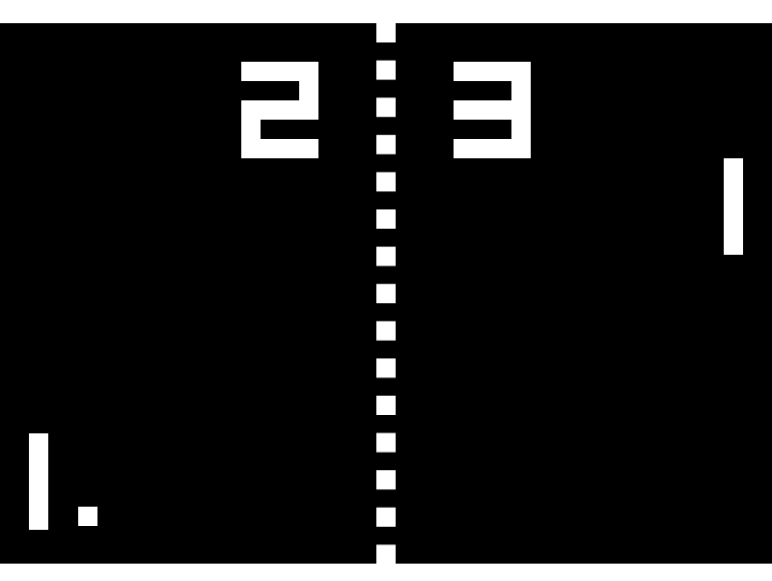
\includegraphics[scale=0.5]{../images/pong.png}
\end{center}
\end{itemize}

\end{document}